% !TEX root = main.tex

\chapter{Introduction}

Attention is all you need~\citep{vaswani2017attention}.
\citet{vaswani2017attention} proposes Transformer.

Use acronyms as follows: this is the first time for \ac{NMT}, and this is the
second time for \ac{NMT}.

\begin{itemize}
    \item Item1
    \item Item2
\end{itemize}

\lipsum[1-2]

\section{Section}

\lipsum[1-2]

\begin{table}[htb]
    \centering
    \caption{Demo table}
    \begin{tabular}{c|c|c}
        cell1 & cell2 & cell3 \\ 
        \hline
        cell4 & cell5 & cell6 \\ 
        cell7 & cell8 & cell9
    \end{tabular}
\end{table}

\subsection{Subsection}

\lipsum[1-2]

\begin{figure}[htb]
    \centering
    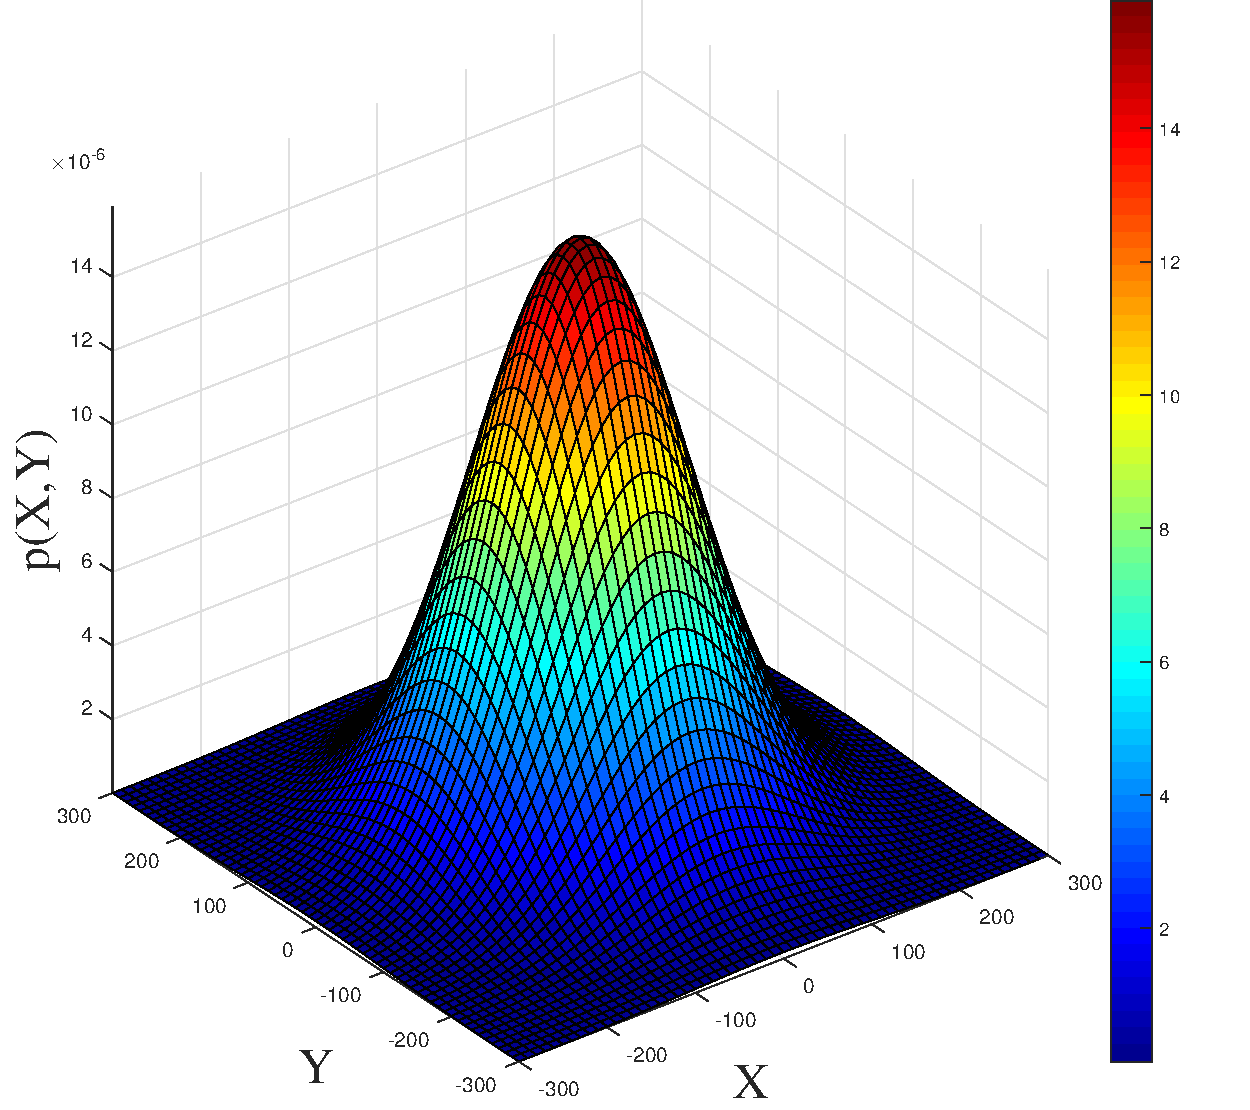
\includegraphics[width=0.5\textwidth]{fig/demo}
    \caption[
    Demo figure: short version
    ]{
        Demo figure: this is a very very very very very very very very very
        very very very very very very very very very very very very very very
        very very very very very very very long caption.
    }
\end{figure}
